%\documentclass[12pt]{article}
%\usepackage{setspace}
%\doublespacing
%\usepackage[margin=0.5in]{geometry}
%\usepackage{rotating} % rotate figures to landscape view
%\usepackage[top=15pt, bottom=10pt, left=20pt, right=20pt]{geometry}
%\usepackage[toc,page]{appendix}
%\usepackage{cancel,comment,alltt}
%\usepackage{mathtools,amsmath,amsthm,bm,amsfonts,amssymb}
%\usepackage{url,hyperref,breakurl}

%\usepackage{float,subfig,color,array,multirow,tikz}

%\usepackage{multirow}
%\linenumbers
%\graphicspath{./}

%\begin{document}
Why convex optimization? 
One of the simplest convex optimization problem is to find the optimum coefficients of a regression function $\hat{y}(x,b) = Ab$, where the functional basis is the column vector of $A$ that spans the space of the functional $\hat{y}(x)$ in it's $x$ domain.
When the optimum coeffients vector $b$ is found, it approximates the true $y(x) = \hat{y}(x,b) + e(x)$ with minimum error.
The minimum error is a convex function defined as 
\begin{equation}
    \epsilon(b) = ||y(x) - \hat{y}(x,b)||_2 = || y - Ab ||_2, 
\end{equation}
the $2$-norm is taken over either discrete sum or continuous integral of $x$.
The $p$-norm is a convex function, hence composing over a affine set gives convexity to $\epsilon(b)$.
Now the optimization problem is to find the $b = [b_1, \cdots, b_n]$ that minimizes $\epsilon(b) \in \mathcal{R}_+$. 


\subsection{Perspective function preserves convex sets}
$f(x,t) = \frac{x}{t}$, where $x \in \mathcal{R}^n$ and $t \in \mathcal{R}_{++}$, and $(x,t)$ is convex.
Given any two sets $(x_1,t_1)$ and $(x_2,t_2)$, the function
$f(\lambda x_1 + (1-\lambda) x_2, \lambda t_1 + (1-\lambda)t_2) = \frac{\lambda x_1 + (1-\lambda)x_2}{\lambda t_1 + (1-\lambda)t_2} = \frac{\lambda t_1}{\lambda t_1 + (1-\lambda)t_2}\frac{x_1}{t_1} + \frac{(1-\lambda)t_2}{\lambda t_1 + (1-\lambda)t_2}\frac{x_2}{t_2} = \nu P(x_1,t_1) + (1-\nu) P(x_2,t_2)$.

The "Perspective of a Function", $f(x,t) = t g(x/t)$, preserving convexity of the convex function $g$, is proven by using the "Perspective function $P$" on the epigraph of $f$ and $g$ as:
epi$f = \{ (x,t,v) \ | \ v \ge f = tg(x/t) \}$ and epi$g = \{ (x/t,v/t) \ | \ v/t \ge g(x/t) \}$, therefore under the same condition $v \ge tg(x/t)$, the perspective function maps epi$f$ to epi$g$, $P(x,t,v) = \frac{(x,v)}{t}$.
Since the perspective function preserves convex sets and epi$g$ is convex by $g$ being convex, hence, epi$f$ must be convex, which indicates a convex $f$. $\blacksquare$ \\

\subsection{Operations that preserve convexity}
\begin{itemize}
\item Nonnegative Weighted Sum of convex functions (viewed as conic set of convex functions (vectors))
\item Composition with an affine mapping
\item Pointwise Maximimum and supremum
\item Composition (with differentiability conditions or without (extended-value extension))
\item Perspective Function
\end{itemize}
\subsubsection{Nonneg Weighted Sum} % do not treat f_i's as differ 
$f = w_1f_1 + w_2 f_2 + \cdots$, where $w_i \ge 0$ and $f_i$'s are convex functions.
Suppose $f(x_2,x_2) = w_1f_1(x_1) + w_2f_2(x_2)$ is a nonnegative weighted sum of two convex functions, then the domain of $f_1$ and $f_2$ doesn't have to be the same.



\subsection{Conjugate function}
\subsubsection{\bf Definition} 
Let $f: R^n \longrightarrow R$. The conjugate function $f^*: R^n \longrightarrow R$ of $f$ is

\begin{equation}
   f^*(y)= \sup_{x \in \text{dom}f}\left( y^T x - f(x) \right).
\end{equation}

\subsubsection{\bf Examples (convex functions)}
\begin{enumerate}
  \item{Affine function} $f(x)= ax+ b$. $yx- ax- b$ is bounded iff $y= a$ (i.e., there exists a supremum over the domain for any given $y$), since the domain is $[-\infty \infty]$, which gives $f^*(y) = -b$.

  \begin{figure}[H]
     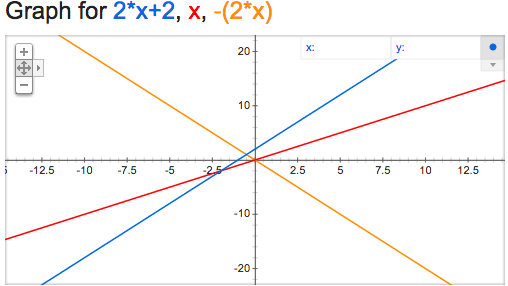
\includegraphics[width=0.5\textwidth]{conj_affine}
  \end{figure}

  \item{Negative logarithm} $f(x)= -\log x$ ($\log$ is the natural $\ln$). $yx+ \log x$  is unbounded if $y\ge 0$, otherwise ($y< 0$) $f^*(y)$ reaches maximum at $x=-1/y$ (set $\frac{\partial f^*(y)}{\partial x}= 0$) , which is $f^*(y)=-\log(-y) - 1$.
  In the figure, $f(y= 1)=x$ (red) and $f(y= -1)=-x$ (orange)

  \begin{figure}[H]
     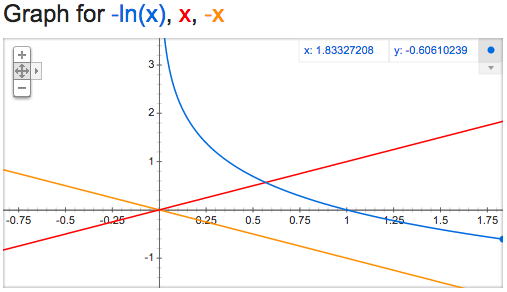
\includegraphics[width=0.5\textwidth]{conj_neg_log}
  \end{figure}

  \item{Exponential} $f(x)= e^x$. $yx- e^x$ is unbounded if $y< 0$, hence when $y> 0$ the maximum is reached at $x= \log y$ with $f^*(y)= y\log y- y$.
	For $y= 0$, $f^*(y)= 0$. 

  \item{Negative entropy} $f(x)= x\log x$ with $\text{dom} f= R_+$.
  
  \begin{figure}[H]   
     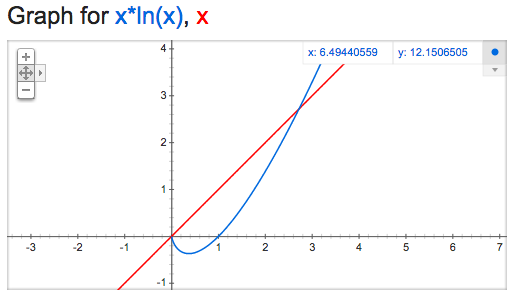
\includegraphics[width=0.5\textwidth]{conj_neg_entropy}
  \end{figure}

  \item{Inverse} $f(x)= 1/x$ on $R_{++}$. $f^*(y\le 0)= -2(-y)^{1/2}$, notice at $y= 0$, the maximum $f^*= 0$ is attained as $x \longrightarrow \infty$, 
  
  \item{Strictly convex quadratic function} $f(x)= \frac{1}{2} x^T Q x$ with $Q\in S_{++}^n$, has the conjugate $f^*= y^Tx - \frac{1}{2} x^T Q x$ which has a maximum at $x= Q^{-1}y$ for all $y$ $\longrightarrow$ $f^*(y)= \frac{1}{2} y^T Q^{-1} y$, where $Q^{-1}$ is also $S_{++}^n$. \\
{\bf Remarks}: The conjugate of a convex quadratic function is also a convex quadratic function.

  \item{Indicator function} $I_S(y)= 0$, $\text{dom}I_S= S$. The conjugate $I_S^*(x)= \sup(y^Tx)$, $y \in C$, is the support function (convex), which gives the pointwise maximum over linear functions of $x$ at any given $x$ (i.e., different $y$ gives different linear functions $y^Tx$ of $x$, so at a point $x_i$, $\sup(y^Tx_i)$ finds the maximum linear function).
  The figure shows three linear functions of $x$ at three different $y=1,2,-3$, so the pointwise maximum function for $x>0$ is at $y=2$. 
  \begin{figure}[H]
     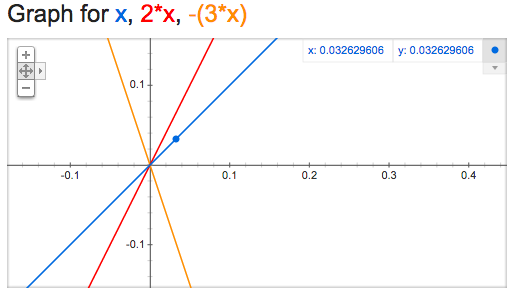
\includegraphics[width=0.5\textwidth]{conj_ind}
  \end{figure}
  
\end{enumerate} 

\subsubsection{\bf Basic Properties}
{\bf Fenchel's inequality} \\
{\bf Conjugate of the conjugate} \\
{\bf Differentiable functions} \\ 
Find the slope of $f(x)$ at $x$, which gives the maximum $x^Ty$ (i.e., $x^T \nabla f(x)$) to pointwise maximize $f^*(y)$!! \\
Conjugate of a differentiable function $f$ $\Rightarrow$ \emph{Legendre transform} of $f$. 
Suppose dom$f= \mathcal{R}^n$, any maximizer $x^*$ of $y^Tx- f(x)$ satisfies $y= \nabla f(x^*)$ (set $\nabla_x f^*(y)=0$).
Therefore, given an arbitrary $x$ satisfying $y= \nabla f(x)$, we can find 
\begin{equation*}
   f^*(y)= x^T \nabla f(x) - f(x).
\end{equation*}
Therefore, the maximized $y$ at $x$ is the slope of both $f(x)$ and the affine function ${x}^Ty$ (passing through the origin). \\
{\bf Scaling and composition with affine transformation} \\
Given $g(x)= af(x)+b$, the conjugate 
\begin{equation*}
   g^*(y)= x^Ty-g(x)= x^Ty-af(x)-b= a(x^T(y/a)-f(x))-b= af^*(y/a)-b.
\end{equation*}
Given $g(x)= f(Ax+b)$, where $A \in \mathcal{R}^{n \times n}$ and $b \in \mathcal{R}^n$, and set $z=Ax+b => x=A^{-1}(z-b)$
\begin{equation*} 
   g^*(y)= x^Ty-g(x)= x^Ty-f(Ax+b)= (A^{-1}(z-b))^Ty-f(z)= z^TA^{-T}y-b^TA^{-T}y-f(z)= f^*(A^{-T}y)-b^TA^{-T}y,
\end{equation*}
dom$g^*=y=A^TA^{-T}y=A^T$dom$f^*$.


\subsection{Quasiconvex Functions}
\subsubsection{Definition}
$f$ is \emph{quasiconvex} if its domain and all its sublevel sets $S_\alpha= \{ x\in $dom$f | f(x) \le \alpha \}$ for $\alpha \in \mathcal{R}$ are convex. \\
$f$ is \emph{quasiconcave} if $-f$ is quasiconvex. \\
$f$ is \emph{quasilinear} if its both quasiconvex and quasiconcave, and all its level sets $S_\alpha= \{ x| f(x)= \alpha \}$ are convex. \\
{\bf Remarks}: Quasiconvex functions can be non-convex, with convex domain and sublevel sets.

\subsubsection{Examples}
\begin{enumerate}
   \item{$\log x$} (Concave function) Both quasiconvex and quasiconcave $\Rightarrow$ quasilinear.
   \item{Ceiling function} (Discontinuous function) $f(x):= \{ z \in \mathcal{Z} | z \ge x, x \in \mathcal{R} \}$ is quasilinear.
   \item{$f(x_1,x_2)= x_1x_2$}(Neither convex nor concave function, Hessian is indefinite; one positive and one negative eigenvalue) $ $dom$f= \mathcal{R}_+^2$, is a quisiconcave function, its superlevel sets $\{x| x_1x_2 \ge \alpha \}$ are convex.
\end{enumerate}

\subsubsection{Basic Properties}
{\bf Jensen's inequality for quasiconvex function}: \\
A function $f$ is quasiconvex $\Leftrightarrow$ dom$f$ is convex and for any $x, y \in $dom$f$ and $0\le \theta \le 1$,
\begin{equation}
   f(\theta x+ (1-\theta)y) \le \max\{f(x), f(y)\}.
\end{equation}
The value of the function on a segment doesn't exceed the maximum of its value at the two endpoints, which could be a non-convex function. (see figure 3.10) \\
{\bf Quasiconvexity by a line intersection}: \\
$f$ is quasiconvex $\Leftrightarrow$ $f$ restricted to a line intersection on its domain is quasiconvex. \\
{\bf Remarks}: \\
A continuous quasiconvex function on $\mathcal{R}$ has a point $c$ in the domain that is a {\bf global minimizer}, and $f$ is nonincreasing and nondecreasing at the left and right of $c$, respectively.

\subsection{Differntiable Quasiconvex Functions}
\subsubsection{1-order conditions}
Suppose $f$ is differentiable.
$f$ is quasiconvex $\Leftrightarrow$ dom$f$ is convex and for all $x$, $y$ $\in$ dom$f$
\begin{equation}
   f(y) \le f(x) \Rightarrow \nabla f(x)^T(y-x) \le 0.
\end{equation}
The definition of quasiconvex function shows that, if $y>x$ ($y<x$) and $f(y) \le f(x)$, $f$ is nonincreasing (nondecreasing) which will always give negative (positive) $\nabla f(x)$.
An analogy to convex function which satisfies $f(y) \ge f(x) + \nabla f(x)^T(y-x)$.
$\nabla f(x)$ defines a supporting hyperplane to the sublevel set $\{ y| f(y) \le f(x) \}$

\subsubsection{2-order conditions}
Suppose $f$ is twice differentiable.
If $f$ is quasiconvex for all $x \in $dom$f$ and all $y \in \mathcal{R}^n$, then if
\begin{equation}
   y^T \nabla f(x)= 0 \Rightarrow y^T \nabla^2 f(x) y \ge 0.
\end{equation}
For a quasifunction on $\mathcal{R}$, this reduces to 
\begin{equation*}
   f'(x)= 0 \Rightarrow f''(x) \ge 0.
\end{equation*}
i.e, whenever the slope is zero, a quasiconvex function has a positive curvature.
For the $\mathcal{R}^n$ case, when $\nabla f(x) \neq 0$ ($y$ is in the $(n-1)$-dim subspace $\nabla f(x)^\perp$ orthogonal (thus independent) to $\nabla f(x)$), $\nabla^2 f(x)$ is positive semidefinite on $\nabla f(x)^\perp$, and have at most one negative eigenvalue in the 1-dim subspace of $\nabla f(x)$.
(proof ommitted)

\subsection{Operations that Preserve Quasiconvexity}
\begin{itemize}
   \item Nonneg weighted maximum
   \item Composition
   \item Minimization
\end{itemize}

\subsubsection{Nonneg weighted maximum}
A nonneg weighted, $w_i \ge 0$ maximum of quasiconvex functions $f_i$,
\begin{equation}
   f(x)= \max\{ w_1f_1(x), \dotsc, w_mf_m(x) \}
\end{equation}
is quasiconvex.
This can be extended to the pointwise supremum of quasiconvex functions $g(x,y)$ for all $y$ ($y$ is like the integer index $i=1,\dotsc,m$, but just in real number space),
\begin{equation}
   f(x)= \sup_{y \in C}\left(w(y)g(x,y)\right).
\end{equation}

\subsubsection{Composition}
\begin{itemize}
   \item If $h \in \mathcal{R}$ nondecreasing, and $g \in \mathcal{R}^n \rightarrow \mathcal{R}$ quasiconvex, then $f= h \circ g$ quasiconvex.
   \item If $f$ quasiconvex, then operating on dom$f$ with affine or linear-fractional transformation on $x$ preserves quasiconvexity. e.g, $f(Ax+b)$ or $f((Ax+b)/(cx+d))$.
\end{itemize}

\subsubsection{Minimization}
Suppose $f(x,y)$ is quasiconvex jointly in $x$ and $y$, and $C$ is convex, then prove that
\begin{equation}
   g(x)= \inf_{y \in C} f(x,y)
\end{equation}
is quasiconvex.
This boils down to proving that the sublevel set $K= \{ x | g(x) \le \alpha \}$ is convex for an arbitrary $\alpha$.
We know that $g(x) \le \alpha \Leftrightarrow f(x,y) \le \alpha + \epsilon$, where $\epsilon > 0$.
Given two points $(x_1,y_1)$ and $(x_2,y_2)$ in the convex sublevel set $\{(x,y) | f(x,y) \le \alpha + \epsilon \}$, with quasiconvexity of $f$,
\begin{equation}
   f(\theta x_1 + (1-\theta)x_2, \theta y_1+ (1-\theta) y_2) \le \alpha + \epsilon.
\end{equation}
By the iff condition,
\begin{equation}
   g(\theta x_1 + (1-\theta)x_2) \le \alpha,
\end{equation}
which implies that $\theta x_1 + (1-\theta)x_2 \in K$, hence $g(x)$ is quasiconvex.

\subsection{Representation via family of convex functions}
The sublevel sets of a quasiconvex function $f$ can be represented by a family of sublevel sets of convex functions,
\begin{equation}
   f(x) \le t \Leftrightarrow \phi_t(x) \le 0.
\end{equation}
i.e., the $t$-sublevel set of $f$ equals the $0$-sublevel set of convex function $\phi$ labeled by $t$.
The figure shows that the blue $f$ given two sublevel $s$ and $t$, where $s\ge t$, then the orange $\phi_s(x)$ is below the red $\phi_t(x)$, $\phi_s(x) \le \phi_t(x)$. 
i.e., due to the $s$-sublevel set of $f$ contains the $t$-sublevel set of $f$, with both sets being convex.
\begin{figure}[H]
   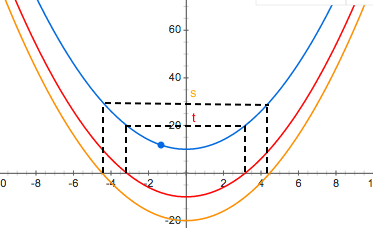
\includegraphics[width=0.5\textwidth]{representation_family_convex_function}
\end{figure}

\subsubsection{Example: Convex over Concave function}
Purpose: A convex over concave function $f$ is quasiconvex, and the {\bf $t$-sublevel sets} could be represented by the $0$-sublevel sets of a family of convex functions (indexed by $t$).\\
Suppose $p(x)$ is convex and $q(x)$ is concave, and $p>0$ and $q>0$ on a convex set $C$, then 
$f(x)=p(x)/q(x)$ is quasiconvex with the relationship
\begin{equation}
   f(x) \le t \Leftrightarrow p(x)-tq(x) \le 0
\end{equation}
which shows that $\phi_t=p(x)-tq(x)$ is convex for $t\le 0$ (i.e., $-q(x)$ is convex).

\section{Log-concave and Log-convex functions}
\subsection{Definition} 
\begin{itemize}
   \item If $f>0$ for all $x \in$ dom$f$, and $\log f(x)$ is concave, then $f$ is a log-concave function.
   \item $f$ is log-convex if log$f$ is convex and $f>0$.
   \item Therefore, $f$ is log-convex iff $1/f$ is log-concave ($-\log f= \log(1/f)$ is concave and $1/f>0$).
   \item Without logarithms, $f$ is log-concave iff $f>0$, dom$f$ is convex, and for all $x, y \in$ dom$f$ and $0\le \theta \le 1$ we have
         \begin{equation}
            f(\theta x+ (1-\theta)y) \ge f(x)^\theta f(y)^{1-\theta}.
         \end{equation}
         If we take $\theta=1/2$, then $f$ at the mean of $x$ and $y$ is at least the geometric mean 
         \footnote{geometric mean of two values is $\sqrt{x_1x_2}$, of three values is $(x_1x_2x_3)^{1/3}$. Measures the central tendency of a set of numbers. 
         The geomtric mean of $x_1$ and $x_2$ gives the edge of a square, which has the same area as a rectangle with the edge of $x_1$ and $x_2$.  } 
         of $f$ at the two points.
\end{itemize}

\subsection{Properties}
\subsubsection{Convexity (concavity) by twice differentiable condition}
Suppose dom$f$ is convex, $f$ is log-convex iff 
\begin{equation}
   \nabla^2 \log f \succeq 0,
\end{equation}
which gives
\begin{equation}
   \frac{1}{f}\nabla^2 f- \frac{1}{f^2}\nabla f \nabla f^T \succeq 0 \Rightarrow f\nabla^2 f \succeq \nabla f \nabla f^T
\end{equation}

\section{Function Convexity wrt Generalized Inequality}
\subsection{Monotonicity wrt generalized inequality}
\subsubsection{$K$-\emph{non-decreasing}}
$f$ is called $K$-\emph{non-decreasing} if $K \subset \mathcal{R}^n$ is a proper cone (convex, solid, pointed, closed), and
\begin{equation}
   x \succeq_K y \Rightarrow f(x) \le f(y).
\end{equation}





%\end{document}


